\subsection{Variational Monte Carlo calculations of the Beryllium and Neon atoms}

	\begin{table}
		\center
			\begin{tabular}{|c|c|c|}
			    \hline
			   	Atom & VMC & References
			    \\ \hline
			    Beryllium & $-14.3888$ & $-14.667$
			    \\ \hline
			    Neon & $-127.961$ &  \(-128.928\)
			    \\	\hline
		  \end{tabular}
		  \caption{Comparison of energies found with Variational Monte Carlo method and
		energies found in research papers \cite{Koput:2011:PCCP} \cite{QUA:QUA560090204} }
		\label{tab:energyReference}
	\end{table}

	We attempt to solve the ground state energy for the Beryllium atom and Neon atom using a Variational Monte Carlo calculation with importance sampling. We have used the trial functions \eqref{eq:BerylliumTrialFunction} for Beryllium and \eqref{eq:NeonTrialFunction} for Neon which uses $\alpha$ and $\beta$ as variational parameters.

	\textbf{NEED TO CALCULATE VALUES AGAIN}

	For Beryllium we have the Alpha and Beta values $\alpha=4.0$ and $\beta=0.31$. We use $10^{6}$ cycles and find the energy to be $-14.3795$, with a variance of $0.0020$.
	For Neon, with $5 \times 10^{5}$ cycles we get an energy of $-127.936$ with a variance of $0.0548$.

	From reseach papers we find the value for energy in the ground state
	of Beryllium to be $-14.667$ \cite{Koput:2011:PCCP} and the value
	for energy in the ground state of Neon to be \(-128.928\) \cite{QUA:QUA560090204}.
	In table \ref{tab:energyReference} we compare results
	obtained with our Variational Monte Carlo method with results from
	various research papers.

	\subsubsection{Alpha and Beta Values}
		\begin{table}
			\center
			\begin{tabular}{| c | c| c |}
			    \hline
			   	\textbf{Trialfunction} & \(\mathbf{\alpha}\) & \(\mathbf{\beta}\)
			    \\ \hline
			    Beryllium $\psi_{T2}$	& 3.8	&	 0.293
			    \\ \hline
			    Neon $\psi_{T2}$	&	10.22	&	0.091
			    \\	\hline
		  \end{tabular}
		  \caption{The values for \(\alpha\) and \( \beta \) where found by doing running Monte Carlo calculation with over a mesh of different \(\alpha\) and \( \beta \) values. For Beryllium each Monte Carlo run went over \(10 000 000\), using importance sampling. For Neon each run went over \(5 000\), also with importance sampling. Then the run with the lowest energy gave the \(\alpha\) and \(\beta\) values.}
		  \label{tab:alpha_beta}
		\end{table}


		\begin{figure}
			\centering 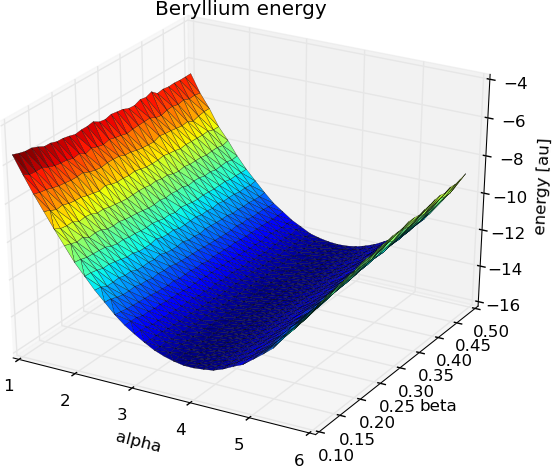
\includegraphics[width=0.45\linewidth]{../figures/Beryllium_alpha_beta_energy}
			\centering 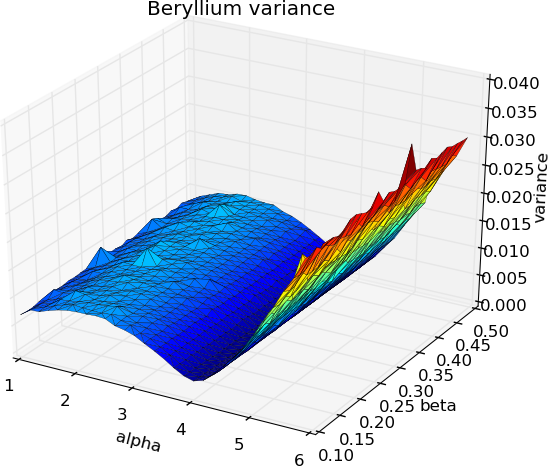
\includegraphics[width=0.45\linewidth]{../figures/Beryllium_alpha_beta_variance}
			\protect\caption{Energy (left) and variance (right) for different Alpha and Beta values for Beryllium, using $10^{6}$ cycles.}
			\label{fig:alpha_beta_comparison_beryllium}
		\end{figure}

		\begin{figure}
			\centering 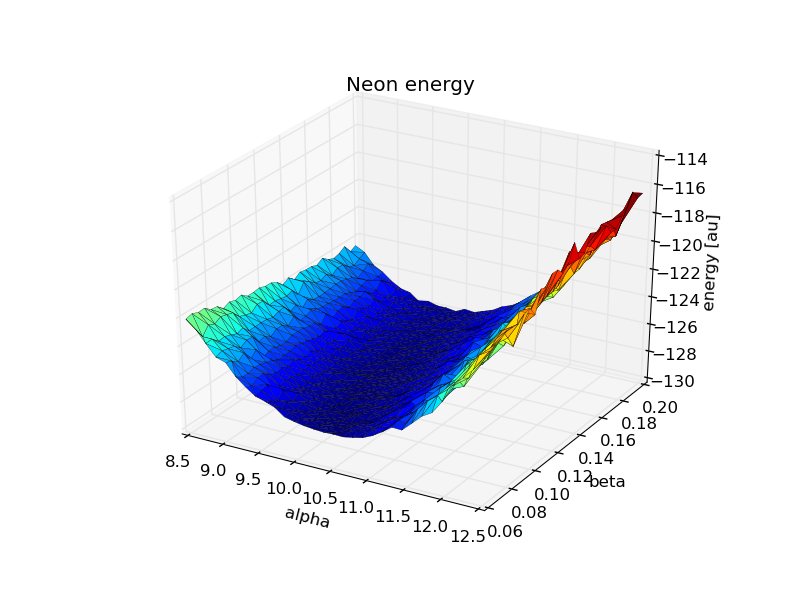
\includegraphics[width=0.45\linewidth]{../figures/Neon_alpha_beta_energy}
			\centering 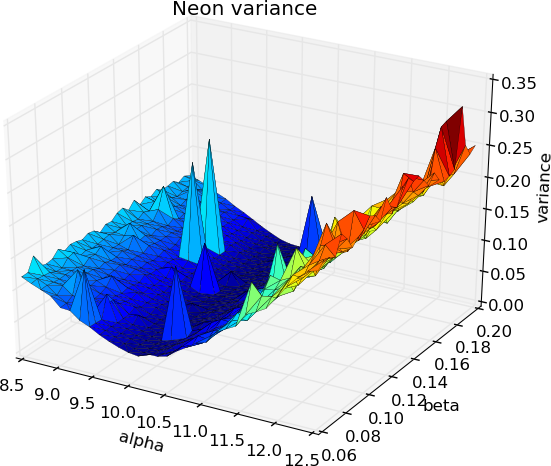
\includegraphics[width=0.45\linewidth]{../figures/Neon_alpha_beta_variance}
			\protect\caption{Energy (left) and variance (right) for different Alpha and Beta values for Neon, using $10^{5}$ cycles.}
			\label{fig:alpha_beta_comparison_neon}
		\end{figure}

		To find optimal Alpha and Beta values for the atoms we run VMC with ranges of different values for \(\alpha\) and \(\beta\). The resulting plots of variance and energy for different combinations are given in figure \ref{fig:alpha_beta_comparison_beryllium} for Beryllium and figure \ref{fig:alpha_beta_comparison_neon} for Neon. The optimal values are shown in table \ref{tab:alpha_beta}. As VMC runs slowly for Neon, because it has 10 electrons, we were only able to run over the range of Alpha and Beta values with $10^{5}$ cycles. This is reflected in the higher variance, and the spikes in the variance plot.


	\subsubsection{Speedup with MPI}
		\begin{table}
			\center
			\begin{tabular}{| c | c| c| c| c|}
				\hline
					\textbf{Num. of processes} &	1	&	2	&	3	&	4
				\\ \hline
				\textbf{Speedup}	&	1.0	&	1.97	&	2.90	&	3.35
				\\	\hline
			\end{tabular}
			\caption{MPI speedup}
			\label{tab:MPI_speedup}
		\end{table}

		\begin{figure}
			\centering 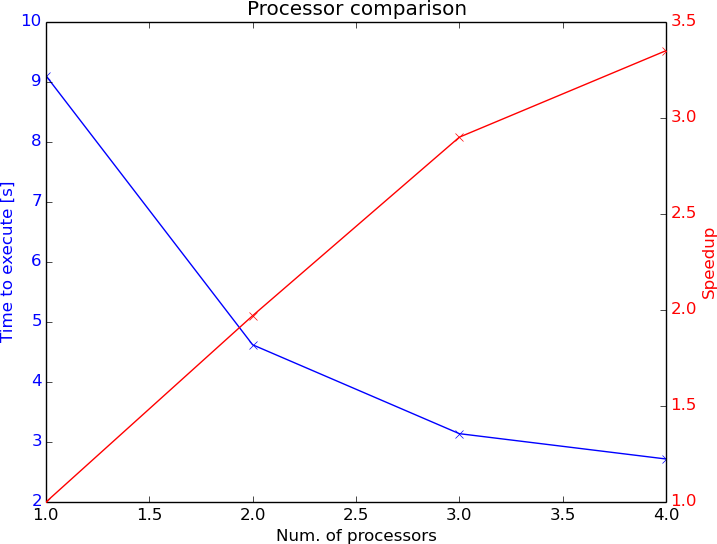
\includegraphics[width=0.45\linewidth]{../figures/processor_number_time_comparison}
			\protect\caption{MPI speedup}
			\label{fig:MPI_speedup}
		\end{figure}

		It is desirable to have a speedup as close as possible to the number of processors used. The speedup measured by our VMC program running 1, 2, 3 and 4 is shown in table \ref{tab:MPI_speedup} and figure \ref{fig:MPI_speedup}. We see that the speedup is good for 2 and 3 processes, but for 4 processes suffers somewhat because it also have to run the OS and other programs.

